\documentclass[12pt,letterpaper]{article}
\usepackage{graphicx,textcomp}
\usepackage{natbib}
\usepackage{setspace}
\usepackage{fullpage}
\usepackage{color}
\usepackage[reqno]{amsmath}
\usepackage{amsthm}
\usepackage{fancyvrb}
\usepackage{amssymb,enumerate}
\usepackage[all]{xy}
\usepackage{endnotes}
\usepackage{lscape}
\newtheorem{com}{Comment}
\usepackage{float}
\usepackage{hyperref}
\newtheorem{lem} {Lemma}
\newtheorem{prop}{Proposition}
\newtheorem{thm}{Theorem}
\newtheorem{defn}{Definition}
\newtheorem{cor}{Corollary}
\newtheorem{obs}{Observation}
\usepackage[compact]{titlesec}
\usepackage{dcolumn}
\usepackage{tikz}
\usetikzlibrary{arrows}
\usepackage{multirow}
\usepackage{xcolor}
\newcolumntype{.}{D{.}{.}{-1}}
\newcolumntype{d}[1]{D{.}{.}{#1}}
\definecolor{light-gray}{gray}{0.65}
\usepackage{url}
\usepackage{listings}
\usepackage{color}

\definecolor{codegreen}{rgb}{0,0.6,0}
\definecolor{codegray}{rgb}{0.5,0.5,0.5}
\definecolor{codepurple}{rgb}{0.58,0,0.82}
\definecolor{backcolour}{rgb}{0.95,0.95,0.92}

\lstdefinestyle{mystyle}{
	backgroundcolor=\color{backcolour},   
	commentstyle=\color{codegreen},
	keywordstyle=\color{magenta},
	numberstyle=\tiny\color{codegray},
	stringstyle=\color{codepurple},
	basicstyle=\footnotesize,
	breakatwhitespace=false,         
	breaklines=true,                 
	captionpos=b,                    
	keepspaces=true,                 
	numbers=left,                    
	numbersep=5pt,                  
	showspaces=false,                
	showstringspaces=false,
	showtabs=false,                  
	tabsize=2
}
\lstset{style=mystyle}
\newcommand{\Sref}[1]{Section~\ref{#1}}
\newtheorem{hyp}{Hypothesis}

\title{Problem Set 2}
\date{Due: October 16, 2022}
\author{Applied Stats/Quant Methods 1}

\begin{document}
	\maketitle
	\section*{Linette Lim}	
	\vspace{.5cm}
	\section*{Question 1 (40 points): Political Science}
		\vspace{.25cm}
	The following table was created using the data from a study run in a major Latin American city.\footnote{Fried, Lagunes, and Venkataramani (2010). ``Corruption and Inequality at the Crossroad: A Multimethod Study of Bribery and Discrimination in Latin America. \textit{Latin American Research Review}. 45 (1): 76-97.} As part of the experimental treatment in the study, one employee of the research team was chosen to make illegal left turns across traffic to draw the attention of the police officers on shift. Two employee drivers were upper class, two were lower class drivers, and the identity of the driver was randomly assigned per encounter. The researchers were interested in whether officers were more or less likely to solicit a bribe from drivers depending on their class (officers use phrases like, ``We can solve this the easy way'' to draw a bribe). The table below shows the resulting data.

\newpage
\begin{table}[h!]
	\centering
	\begin{tabular}{l | c c c }
		& Not Stopped & Bribe requested & Stopped/given warning \\
		\\[-1.8ex] 
		\hline \\[-1.8ex]
		Upper class & 14 & 6 & 7 \\
		Lower class & 7 & 7 & 1 \\
		\hline
	\end{tabular}
\end{table}

\begin{enumerate}
	
	\item [(a)]
	Calculate the $\chi^2$ test statistic by hand/manually (even better if you can do "by hand" in \texttt{R}).\\
	\vspace{7cm}
	
	\item
Answer for Question 1a\\
\noindent First, make sure global environment is empty, load packages such as Tidyverse, and set the working directory.\\ 
\noindent Now create data in R using the following code:\\
\vspace{.5cm}
\lstinputlisting[language=R, firstline=7, lastline=29]{PS2_answers_LL.R}  
\vspace{.5cm}
\noindent We get a matrix, A:\\
\begin{verbatim}
            Not stopped Bribe requested Stopped or warned
Upper class          14               6                 7
Lower class           7               7                 1
\end{verbatim}            
\noindent I manually calculated the row and column totals using these steps:\\
\vspace{.5cm}
\lstinputlisting[language=R, firstline=32, lastline=39]{PS2_answers_LL.R}  
\vspace{.5cm}
\noindent Based on the row and column totals, I created a new matrix with the following code:\\
\vspace{.5cm}
\lstinputlisting[language=R, firstline=41, lastline=63]{PS2_answers_LL.R}  
\vspace{.5cm}
\noindent The new matrix, B, is as follows:\\
\begin{verbatim}
             Not stopped Bribe requested Stopped or warned Row total
Upper class           14               6                 7        27
Lower class            7               7                 1        15
Column total          21              13                 8        42
\end{verbatim}
\vspace{.3cm}
\noindent Now, I calculate the Fe, or Fexpected with the formula Fe = (Row total / grand total) * column total, and with that we can calculate the chi square statistic:\\
\vspace{.5cm}
\lstinputlisting[language=R, firstline=69, lastline=76]{PS2_answers_LL.R}  
\vspace{.5cm}
\ The chi square is:\\
\begin{verbatim}
[1] 3.791168
\end{verbatim}
\vspace{.3cm}
\noindent To check if the answer 'by hand' is correct, we can run the chisq.test() function on A and we get chi square = 3.7912:\\
\begin{verbatim}
	Pearson's Chi-squared test

data:  A
X-squared = 3.7912, df = 2, p-value = 0.1502
\end{verbatim}
\vspace{.3cm}

	\item [(b)]
	Now calculate the p-value from the test statistic you just created (in \texttt{R}).\footnote{Remember frequency should be $>$ 5 for all cells, but let's calculate the p-value here anyway.}  What do you conclude if $\alpha = 0.1$?\\
	
		\item
Answer for Question 1b\\
\noindent First, we calculate the degrees of freedom with the formula: df = (rows -1)(columns -1). We get df=2. We then use df=2 in the following formula to find the p-value:\\
\vspace{.5cm}
\lstinputlisting[language=R, firstline=89, lastline=89]{PS2_answers_LL.R}  
\vspace{.5cm}
\noindent We get:\\
\begin{verbatim}
[1] 0.1502306
\end{verbatim}
\noindent To confirm if p-value is 0.15, I convert the matrix (A) created earlier into a table and run some code as follows. The summary() function reaffirms the chi sq statistic as 3.79 and the p-value as 0.15.\\
\vspace{.5cm}
\lstinputlisting[language=R, firstline=96, lastline=98]{PS2_answers_LL.R}  
\vspace{.5cm}
\noindent The output is as follows:\\
\begin{verbatim}
> summary(table)
Number of cases in table: 42 
Number of factors: 2 
Test for independence of all factors:
	Chisq = 3.791, df = 2, p-value = 0.1502
	Chi-squared approximation may be incorrect
\end{verbatim}
\noindent The p-value is 0.15. This is larger than the significance level alpha = 0.1, so we do not have enough evidence to reject the null hypothesis, that there is no relationship between the two variables, socioeconomic class and treatment by police officers.\\
	
	\newpage
	\item [(c)] Calculate the standardized residuals for each cell and put them in the table below.
	\vspace{1cm}
	
	\begin{table}[h]
		\centering
		\begin{tabular}{l | c c c }
			& Not Stopped & Bribe requested & Stopped/given warning \\
			\\[-1.8ex] 
			\hline \\[-1.8ex]
			Upper class  &  &  &  \\
			\\
			Lower class &  &   &   \\
			
		\end{tabular}
	\end{table}
			\item
Answer for Question 1c\\
\noindent To access the standardized residuals, you can assign the output of your chisq.test() to an object, and print out using object\$stdres:\\
\vspace{.5cm}
\lstinputlisting[language=R, firstline=108, lastline=109]{PS2_answers_LL.R}  
\vspace{.5cm}
\noindent We get:\\
\begin{verbatim}
> model$stdres
            Not stopped Bribe requested Stopped or warned
Upper class   0.3220306      -1.6419565         1.5230259
Lower class  -0.3220306       1.6419565        -1.5230259
\end{verbatim}
\noindent It is also possible to calculate by hand in r. First, we calculate the row and column proportions:\\
\vspace{.5cm}
\lstinputlisting[language=R, firstline=114, lastline=125]{PS2_answers_LL.R}  
\vspace{.5cm}
\noindent Next, we can find out the standardized residuals using the following formula:\\
\vspace{.5cm}
\lstinputlisting[language=R, firstline=129, lastline=134]{PS2_answers_LL.R}  
\vspace{.5cm}
\noindent Finally using the same formula earlier for creating matrix A and B, we can arrange the standardized residuals for each cell in another matrix, C. You can see we have arrived at the same standardized residuals through calculation by hand in R.\\
\begin{verbatim}
> print(C)
            Not stopped Bribe requested Stopped or warned
Upper class   0.3220306       -1.641957          1.523026
Lower class  -0.3220306        1.641957         -1.523026
\end{verbatim}
	
	\vspace{7cm}
	\item [(d)] How might the standardized residuals help you interpret the results?  
	
			\item
Answer for Question 1d\\
\noindent First, we create a dataframe so that it is easier to manipulate the data with ggplot.\\
\vspace{.5cm}
\lstinputlisting[language=R, firstline=165, lastline=171]{PS2_answers_LL.R}  
\vspace{.5cm}
\noindent We get:\\
\begin{verbatim}
> print(dataframe)
  Class Cases       Treatment
1 upper    14     not.stopped
2 upper     6 bribe.requested
3 upper     7  stopped.warned
4 lower     7     not.stopped
5 lower     7 bribe.requested
6 lower     1  stopped.warned
\end{verbatim}
\noindent Next, we apply the ggplot() function.\\
\vspace{.5cm}
\lstinputlisting[language=R, firstline=173, lastline=179]{PS2_answers_LL.R}  
\vspace{.5cm}
\begin{figure}[hbtp!]\centering
	\caption{\footnotesize Relationship between Class and Police treatment.}
	\label{fig:plot_1}
	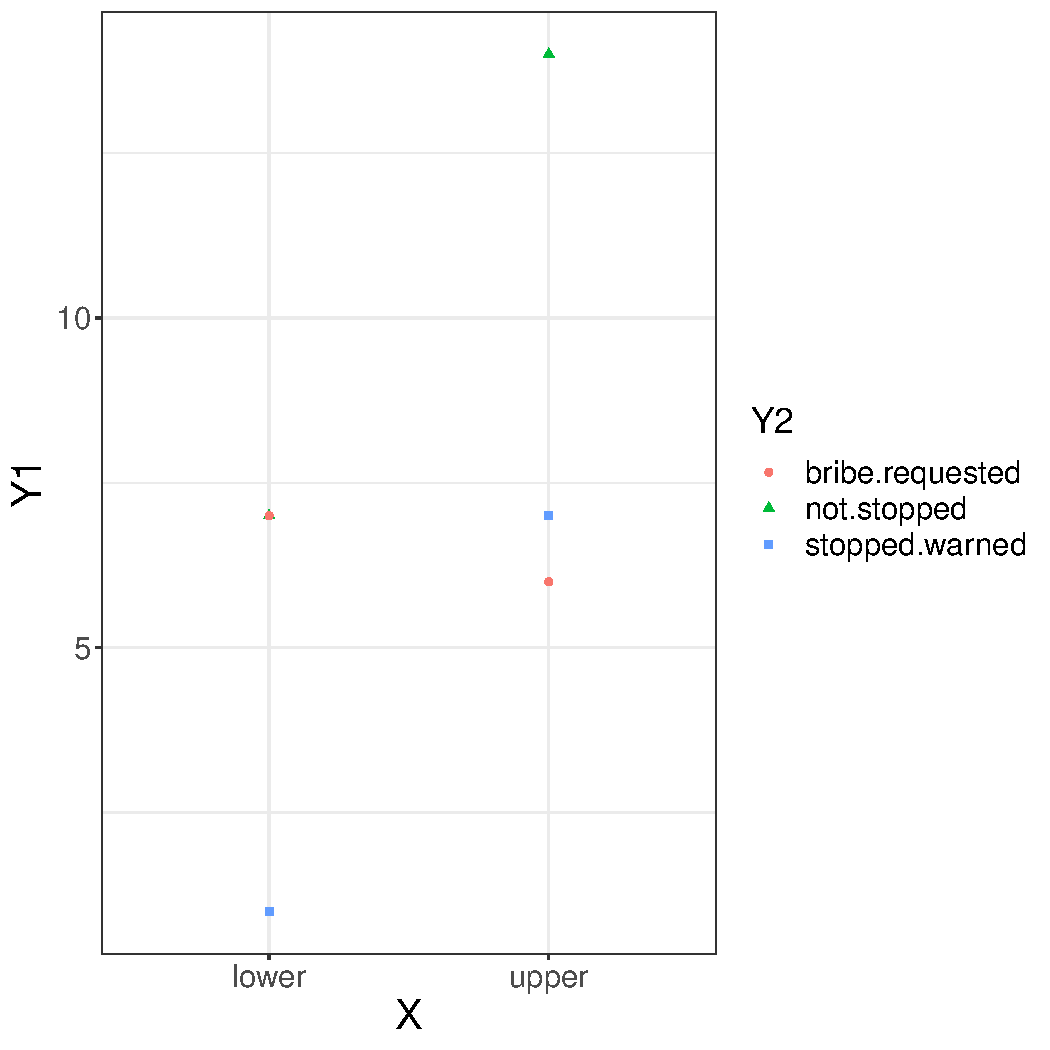
\includegraphics[width=.75\textwidth]{plot_class_treatment.pdf}
\end{figure}
\noindent Based on plot 1, we see that both classes have a similar likelihood of being targeted for bribes. It also looks like (a) the upper class are more likely to be not stopped when flouting traffic rules. However, it seems puzzling that at the same time, (b) a member of the upper class is also more likely to be stopped or warned than someone deemed lower class. Since the interpretation is unclear, let us try using standardized residuals to interpret the results. We use the following formula:\\
\vspace{.5cm}
\lstinputlisting[language=R, firstline=210, lastline=212]{PS2_answers_LL.R}  
\vspace{.5cm}
\begin{figure}[hbtp!]\centering
	\caption{\footnotesize Relationship between Class and Police treatment.}
	\label{fig:plot_1}
	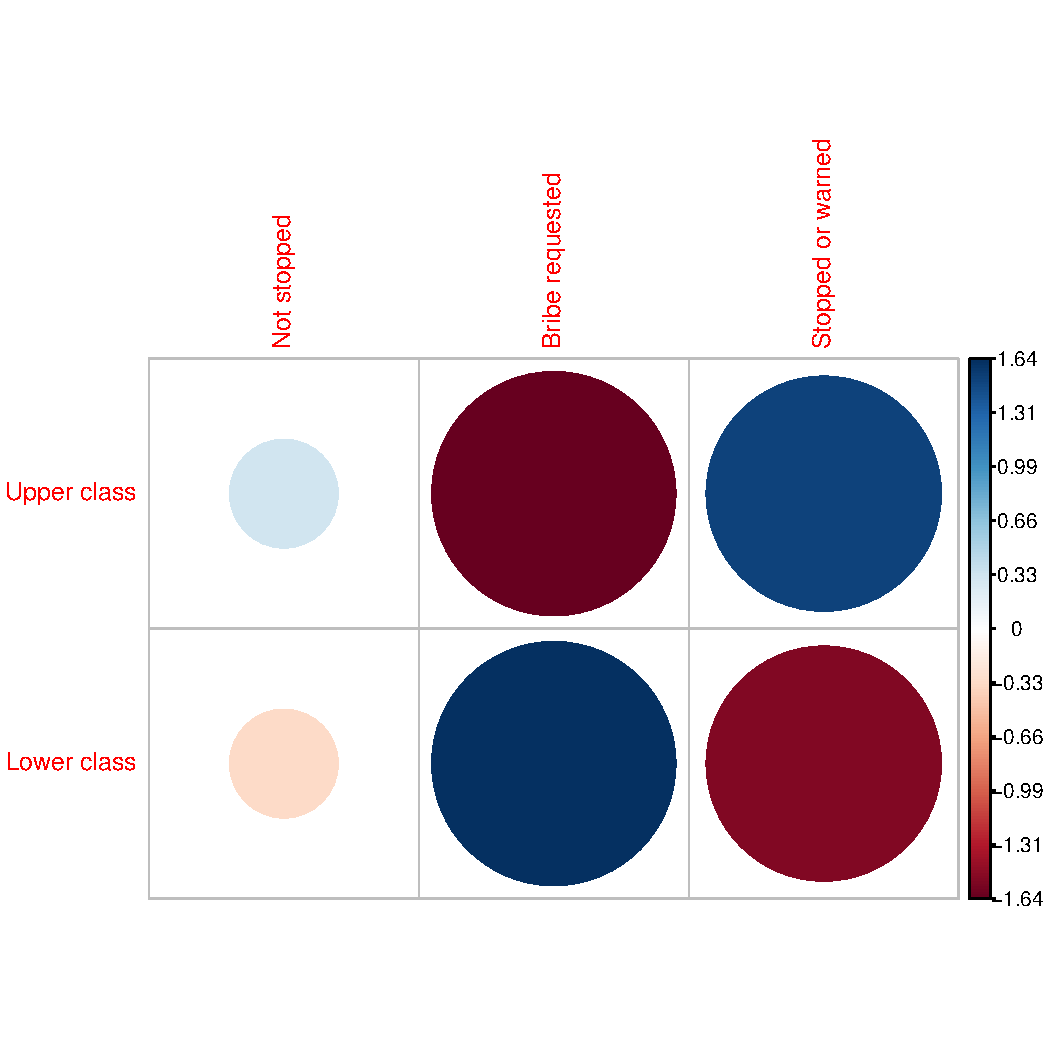
\includegraphics[width=.75\textwidth]{corrplot_class_treatment.pdf}
\end{figure}
\noindent Conclusion: The positive residuals are in blue, signifying a positive association between the corresponding row and column variables. In the plot, we can see a strong positive association between being lower class and being asked to pay a bribe. There is also a strong positive association between being upper class and being stopped or warned. This seems to suggest that the lower class are often stymied by 'informal' ways of doing things, possibly due to a combination of low social capital and lack of literacy in the law, while the upper class are somewhat protected by and benefit from formal institutions like the law and the police force.\\
\noindent The negative residuals are in red. This implies a negative association between the corresponding row and column variables. From the plot, we see the upper class  is less likely (or 'not associated' with) to be asked to pay a bribe, while the  lower class is less likely to be stopped or warned. Taken together, this suggests that there are different traffic offense resolution methods for the upper class and the lower class. The lower class is more usually let go with a bribe, while the upper class is more likely to be formally warned or sanctioned.\\
	
\end{enumerate}
\newpage

\section*{Question 2 (40 points): Economics}
Chattopadhyay and Duflo were interested in whether women promote different policies than men.\footnote{Chattopadhyay and Duflo. (2004). ``Women as Policy Makers: Evidence from a Randomized Policy Experiment in India. \textit{Econometrica}. 72 (5), 1409-1443.} Answering this question with observational data is pretty difficult due to potential confounding problems (e.g. the districts that choose female politicians are likely to systematically differ in other aspects too). Hence, they exploit a randomized policy experiment in India, where since the mid-1990s, $\frac{1}{3}$ of village council heads have been randomly reserved for women. A subset of the data from West Bengal can be found at the following link: \url{https://raw.githubusercontent.com/kosukeimai/qss/master/PREDICTION/women.csv}\\

\noindent Each observation in the data set represents a village and there are two villages associated with one GP (i.e. a level of government is called "GP"). Figure~\ref{fig:women_desc} below shows the names and descriptions of the variables in the dataset. The authors hypothesize that female politicians are more likely to support policies female voters want. Researchers found that more women complain about the quality of drinking water than men. You need to estimate the effect of the reservation policy on the number of new or repaired drinking water facilities in the villages.
\vspace{.5cm}	

\newpage
\begin{enumerate}
	\item [(a)] State a null and alternative (two-tailed) hypothesis. 
	
				\item
Answer for Question 2a\\
\noindent First, we clear the global environment, load packages, set the working directory, and import the data.\\
\vspace{.5cm}
\lstinputlisting[language=R, firstline=237, lastline=240]{PS2_answers_LL.R}  
\vspace{.5cm}
\noindent Let us find the difference in means for the number of drinking water facilities between the villages with treatment (reservation for women) and without treatment using this formula:\\
\vspace{.5cm}
\lstinputlisting[language=R, firstline=242, lastline=242]{PS2_answers_LL.R}  
\vspace{.5cm}
\noindent We get:\\
\begin{verbatim}
[1] 9.252423
\end{verbatim}
\noindent Thi suggests that the reservation policy increased the number of drinking water facilities in a GP on average by about 9 (new or repaired). Therefore, the null hypothesis is that there is zero treatment effect, i.e.:\\
\vspace{.5cm}
\lstinputlisting[language=R, firstline=248, lastline=249]{PS2_answers_LL.R}  
\vspace{.5cm}
	
	\vspace{6cm}
	\item [(b)] Run a bivariate regression to test this hypothesis in \texttt{R} (include your code!).
					\item
Answer for Question 2b\\
\noindent We run a bivariate regression using the lm() function:\\
\vspace{.5cm}
\lstinputlisting[language=R, firstline=252, lastline=254]{PS2_answers_LL.R}  
\vspace{.5cm}
\noindent We get:\\
\begin{verbatim}
Call:
lm(formula = water ~ reserved, data = data)

Residuals:
    Min      1Q  Median      3Q     Max 
-23.991 -14.738  -7.865   2.262 316.009 

Coefficients:
            Estimate Std. Error t value Pr(>|t|)    
(Intercept)   14.738      2.286   6.446 4.22e-10 ***
reserved       9.252      3.948   2.344   0.0197 *  
---
Signif. codes:  0 ‘***’ 0.001 ‘**’ 0.01 ‘*’ 0.05 ‘.’ 0.1 ‘ ’ 1

Residual standard error: 33.45 on 320 degrees of freedom
Multiple R-squared:  0.01688,	Adjusted R-squared:  0.0138 
F-statistic: 5.493 on 1 and 320 DF,  p-value: 0.0197
\end{verbatim}
\noindent Here, we see that the p-value = 0.0197. This is less than the typical threshold of alpha=0.05, so we reject the null hypothesis that treatment effect (of reservation policy on new or repaired drinking water facilities) is zero.\\

	\vspace{6cm}
	\item [(c)] Interpret the coefficient estimate for reservation policy. 
						\item
Answer for Question 2c\\
\noindent From the output above, we can see that the coefficient estimate for reservation policy is 9.252, the standard error is 3.948, and the t-statistic for the estimated slope coefficient is 2.344. The slope coefficient is equal to the difference-in-means estimator earlier calculated (9.252423). When the  explanatory variable is binary, the estimated average treatment effect equals the estimated slope coefficient. We can run the confint() function to check:\\
\vspace{.5cm}
\lstinputlisting[language=R, firstline=262, lastline=262]{PS2_answers_LL.R}  
\vspace{.5cm}
\noindent We get:\\
\begin{verbatim}
> confint(fit.data)
                2.5 %   97.5 %
(Intercept) 10.240240 19.23640
reserved     1.485608 17.01924
\end{verbatim}
\noindent The result tells us that having reservations for women is estimated to increase the number of drinking water facilities by 9.25 facilities with a 95 percent confidence interval of [1.49, 17.02].\\

\end{enumerate}

\end{document}
